documentclass{standalone}
\usepackage{tikz}
\usetikzlibrary{shapes,arrows}
\usepackage[utf8]{inputenc}

\tikzstyle{block} = [rectangle, draw, fill=blue!20, 
    text width=5em, text centered, rounded corners, minimum height=4em]
\tikzstyle{line} = [draw, -latex']
\tikzstyle{cloud} = [draw, ellipse,fill=red!20, node distance=3cm,
    minimum height=2em]

\begin{document}
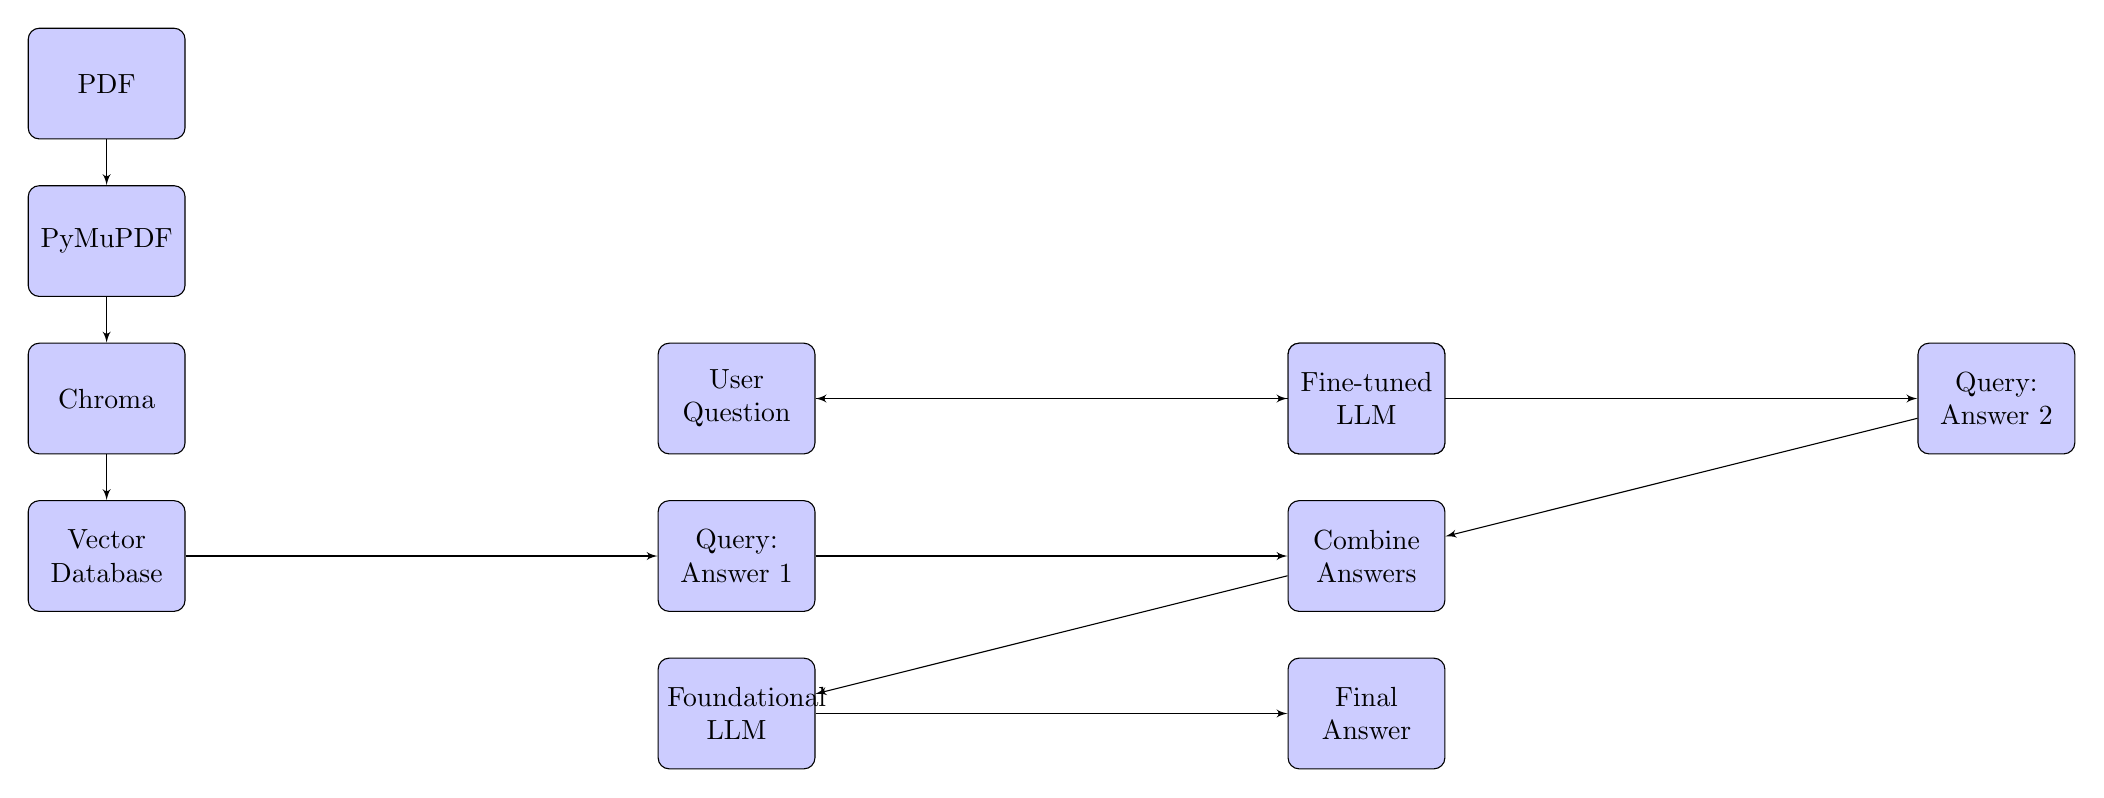
\begin{tikzpicture}[node distance = 2cm, auto]
\node[block] (pdf) {PDF};
\node[block, below of=pdf] (pymupdf) {PyMuPDF};
\node[block, below of=pymupdf] (chroma) {Chroma};
\node[block, below of=chroma] (vecdb) {Vector Database};
\node[block, right of=vecdb,xshift=6cm] (qa1) {Query: Answer 1};
\node[block, right of=qa1,xshift=6cm] (combined) {Combine Answers};
\node[block, below of=qa1] (llm) {Foundational LLM};
\node[block, below of=combined] (finalanswer) {Final Answer};
\node[block, right of=chroma,xshift=6cm] (userq) {User Question};
\node[block, right of=userq,xshift=6cm] (dataload) {Data Processing};
\node[block, right of=dataload,xshift=6cm] (qna) {Query: Answer 2};
\node[block, right of=userq,xshift=6cm] (llmfinetuned) {Fine-tuned LLM};

\path[line] (pdf) -- (pymupdf);
\path[line] (pymupdf) -- (chroma);
\path[line] (chroma) -- (vecdb);
\path[line] (vecdb) -- (qa1);
\path[line] (qa1) -- (combined);
\path[line] (combined) -- (llm);
\path[line] (llm) -- (finalanswer);
\path[line] (dataload) -- (userq);
\path[line] (userq) -- (llmfinetuned);
\path[line] (llmfinetuned) -- (qna);
\path[line] (qna) -- (combined);

\end{tikzpicture}
\end{document}